\section{Antenna}\label{sec:antenna}

Based on the overview of the system made in Chapter \ref{ch:uas}, a modelling of the radiation pattern of the directional antenna is in due to be able to simulate the scenario.

The radiation patterns are a graphical way of representing the radiation properties of the antenna as a function of space. These patterns are very useful when it comes to how an antenna perform. As an example, figure \ref{fig:radpattern} shows the radiation patterns of a real directional antenna.

\begin{figure}[H]
	\centerline{
	\includegraphics[scale=0.45]{figures/radpattern.png}}
	\caption{Radiation Pattern of a real directional antenna.}
	\label{fig:radpattern}
\end{figure}

\paragraph{}Note how, for a 3 dimensional radiation pattern, 2 planes are defined. These are the horizontal plane (H-plane) and the vertical plane (V-plane). For simplicity, during this project it is assumed that the radiation pattern is symmetric, and therefore, exactly the same for both planes.

\paragraph{}The concentric circles inside the plot represent the normalized power radiated in decibels (even though it is possible to find non-normalized plots as well). The closer to the center the circles are, the weaker the power gets in a logaritmic scale.

\paragraph{}Choosing the parabolic and the patch antennas showed in table \ref{table:1} a radiation pattern was build by using the mathematical function \textit{sinc}, as shown in figure \ref{fig:sinc}.

\begin{table}[h]
	\centering
	\begin{tabular}{|c||c|c|}
		\hline
		Parameter & GS & UA\\ \hline\hline
		Type & Parabolic & Patch\\ \hline
		Polarization & Linear & Linear\\ \hline
		Frequency [GHz] & $2.4$ & $2.4$\\ \hline
		Gain [dB] & $24$ & $14$\\ \hline
		HPBW/$H(^{\circ})$ & $14$ & $45$\\ \hline
		HPBW/$V(^{\circ})$ & $10$ & $45$\\ \hline
	\end{tabular}
	\caption{Table of antennas parameters}
	\label{table:1}
\end{table}

\begin{figure}[H]
\hfill
\subfigure[Sinc function natural units.]{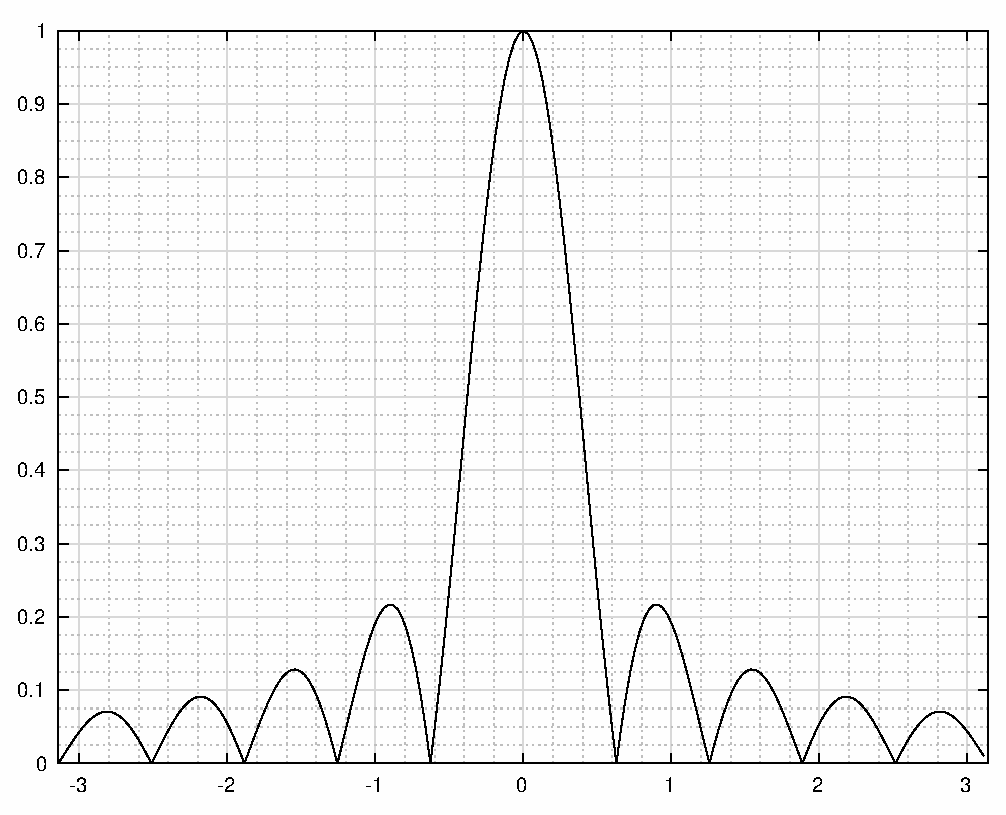
\includegraphics[scale=0.4]{figures/sinc1.eps}}
\hfill
\subfigure[Sinc function logaritmic units.]{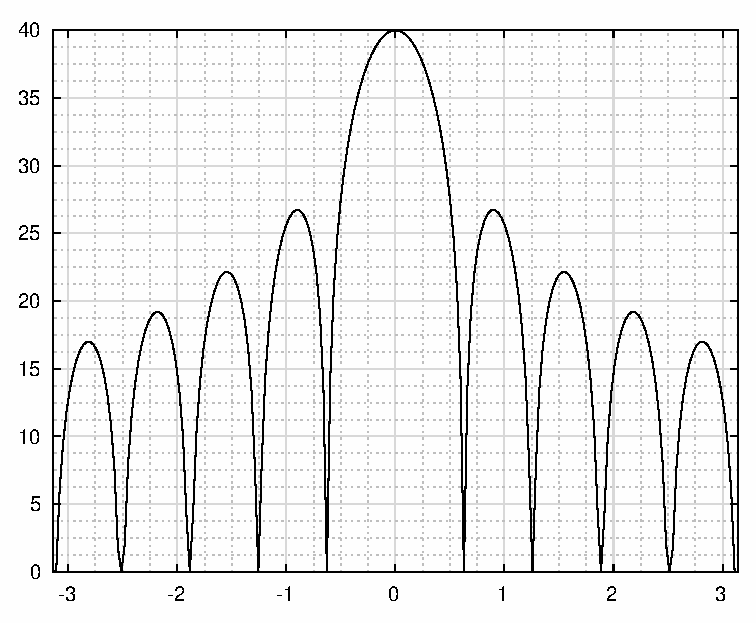
\includegraphics[scale=0.4]{figures/sinc2.eps}}
\hfill
\caption{Sinc function.}
\label{fig:sinc}
\end{figure}

Plotting this \textit{sinc} in a form of a radiation pattern, similar features of a real antenna can be achieved (figure \ref{fig:radiationpattern}).

\begin{figure}[H]
	\centering
	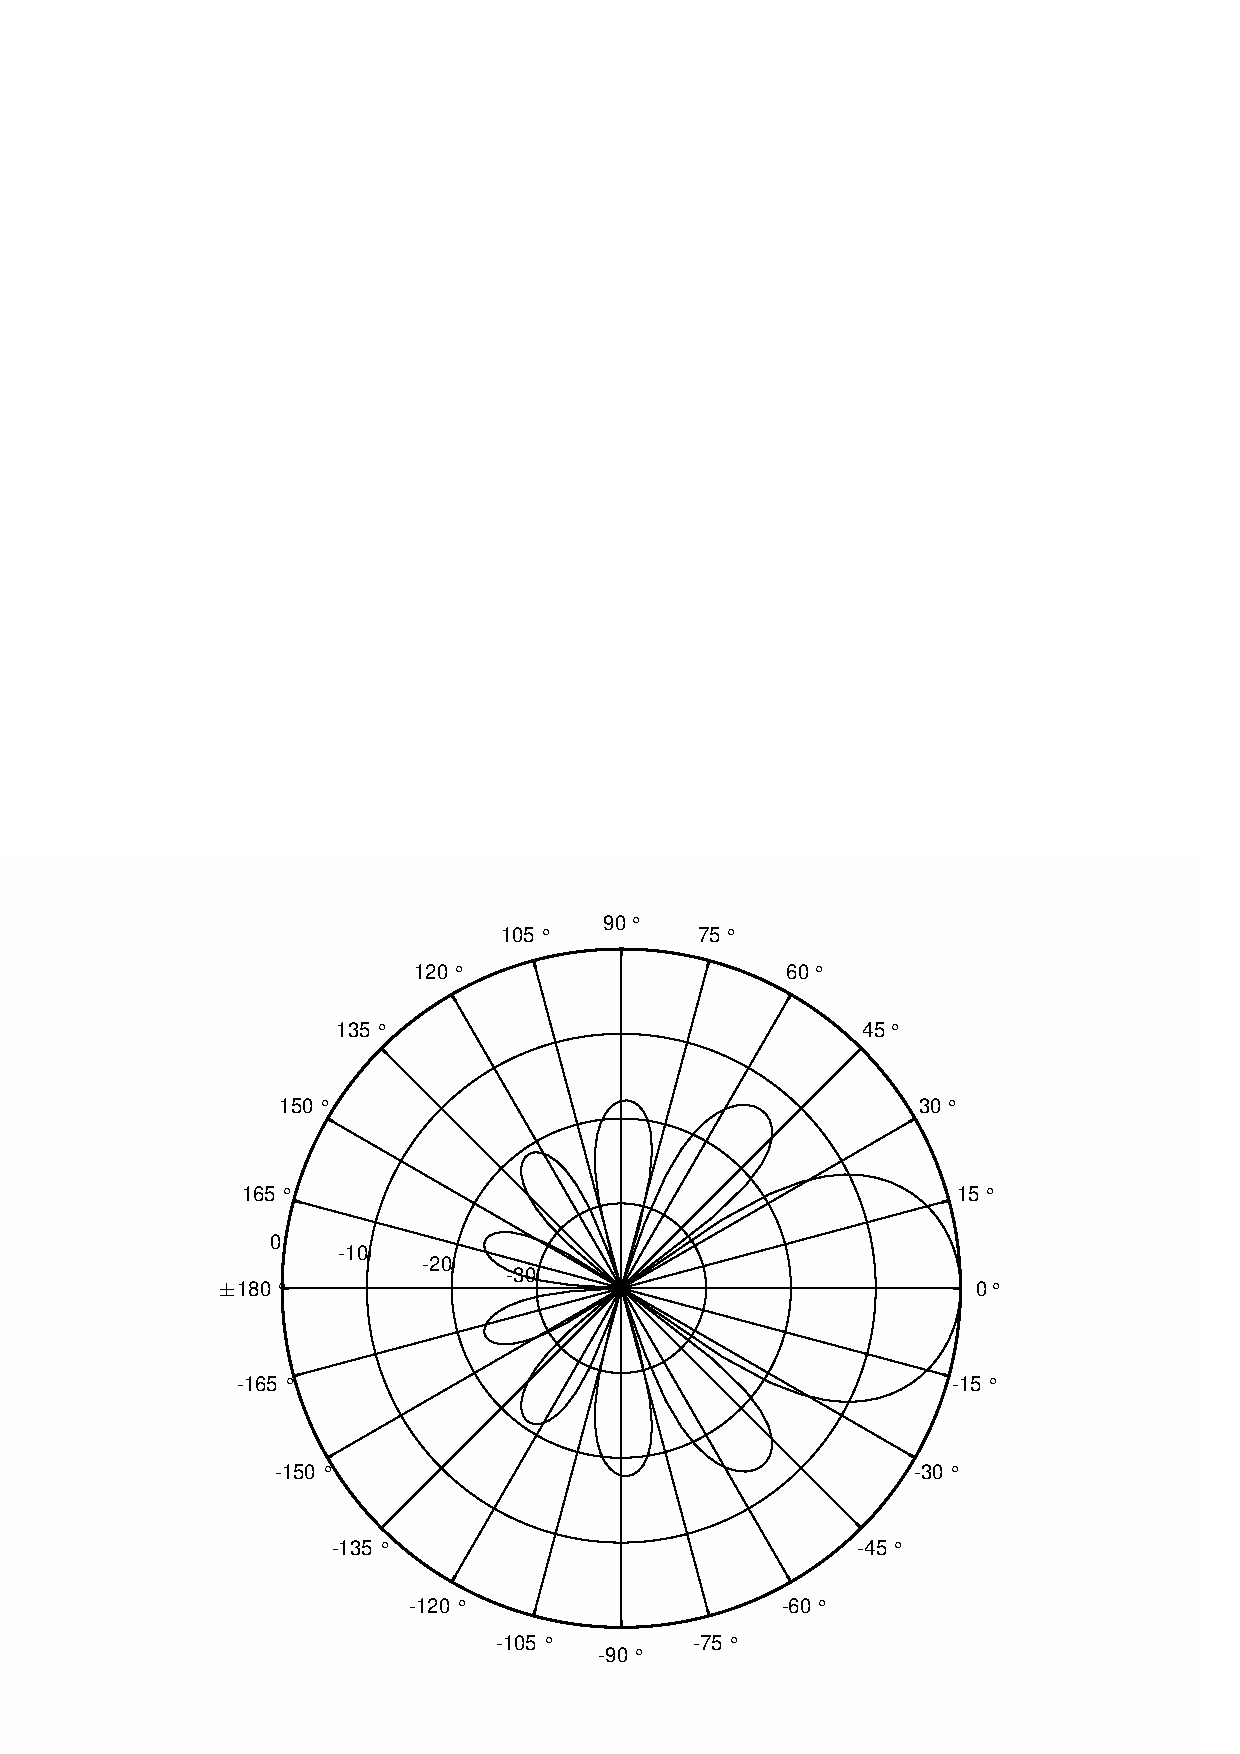
\includegraphics[scale=0.6]{figures/radiationpattern.png}
	\caption{Radiation Pattern based on sinc.}
	\label{fig:radiationpattern}
\end{figure}
